\section{Estimation}

Only a single parameter of the model needs to be estimated: $\beta_L$. For this estimation, method of simulated moments is employed.  \textcite{eisenhauer_estimation_2015} suggests a diagonal matrix is a standard choice as weight matrix when using methods of moments, allowing for writing the estimation as the sum of squared errors of the simulated and empirical moments. Phrased differently: the objective function minimizes the mean squared error (MSE) between the empirical moments and the simulated. The procedure goes: Simulate $N$ individuals and find the relevant moments of the supplied working hours. Since I use aggregate data from Statistics Denmark, I have not access to the standard errors of the estimates, usually used for the weight of the individual moments. Instead I weigh each moment equally. Since this application relies on grid search over the single parameter $\beta_L$, I choose the $\beta_L$ corresponding to the lowest loss with regards to the objective function. 

Usually when estimating a structural model, using simulated methods of moments one would supply the parameters not as part of the state space. The reason for this, is that as the size of the state space expands, it gets exponentially more expensive to solve the model. The algorithm would go: For a given set of parameters needed to be estimated, supply a random initialization. Solve the model for given parameters. Use the solved model to calculate the moments. Use numerical optimization to minimize given optimization problem. However in this application I have chosen to make the parameter part of the state space, since this paper tries to establish that high dimensional dynamic models can be solved using Deep Reinforcement Learning, and therefore not being a limited by the size of the state space.

This paper has implemented the following strategy for estimating the model: I create a grid of 50 points with $\beta_L$ values in the range $[0.2, 8]$ evenly spaced. I simulate $N=300$ agents for a given value of $\beta_L$ in the grid. Using the 300 agents i can calculate the mean number of supplied hours pr. agent. Here it is important to note, that if an agent works 0 hours, the agent is assumed to be out of the workforce and not appear in the statistics, therefore the objective function is:

\begin{equation}
    \text{Objective} = \sum_{q=Q_{\min}}^{Q_{\max}} \lsp \mu_{q} -\frac{1}{\sum_{i=1}^{N} \mathbf{1}\{H_{i,q} > 0\}}\sum_{i=1}^N (H_{i,q})\rsp^2
\end{equation}

where $q$ denotes the age of an individual agent and $i$ denotes an individual. $\mu_q$ is the true average number of supplied ours of women at given age. Again I use \textbf{LIGEF15} supplied by Statistics Denmark to get the numbers of average supplied number of hours. I use the same seed for the simulation, every time the $N$ agents is simulated with a new $\beta_L$ value. The estimation is performed for each of the solution methods in this paper: Value function Iteration, Deep Q-Learning and Double Deep Q-Learning. 

The estimation yields the following optimal values using VFI: $\beta_L=3.43$, Optimal Values using DQN $\beta_L=3.59$ and optimal value of Double DQN $\beta_L=3.59$. $3.43$ and $3.59$ are neighbouring grid points. I believe it's safe to conclude that these methods yields if not identical, then almost identical results, and I am willing to conclude that using Deep Q-Learning of Double Deep Q-Learning is excellent methods for solving dynamic models - at least in this setting!

\begin{table}[ht]
    \centering
    \begin{tabular}{lrrr}
\toprule
{} &  VFI &  DQN & Double DQN \\
\midrule
$\hat{\beta_L}$ & 3.43 & 3.59 & 3.59 \\
\bottomrule
\end{tabular}
    \caption{Estimation of $\beta_L$}
    \label{tab:beta_L_Estimation}
\end{table}

Looking to figure \ref{fig:beta_L_estimation} it can be seen that the estimations follow the same trajectory. The plot shows the log(MSE) for $\beta_L$ values in the range $[0.2, 8]$. Starting with low $\beta_L$ having medium high MSE, falling slightly at around a $\beta_L = 3$ reaching a minimum at about $\beta_L = 3.5$, and after that a sharp raise in MSE is observed. 

\begin{figure}[ht]
\begin{subfigure}{.5\textwidth}
  \centering
  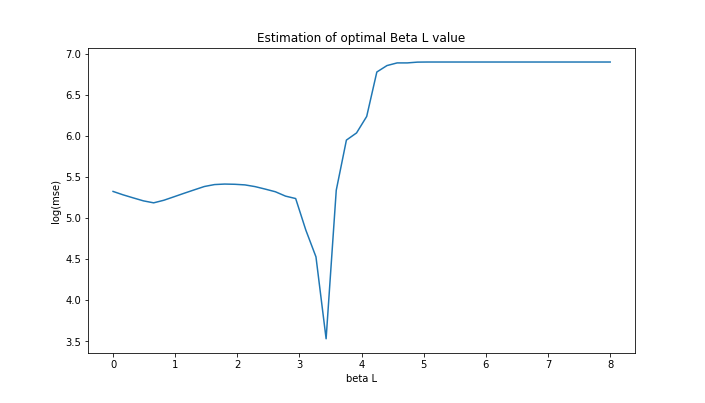
\includegraphics[width=1\linewidth]{figures/dqi_model1_estimation_Beta_L.png}
  \caption{Value Function Iteration Estimation of $\beta_L$}
  \label{fig:dqi_estimation_beta_L}
\end{subfigure}%
\begin{subfigure}{.5\textwidth}
  \centering
  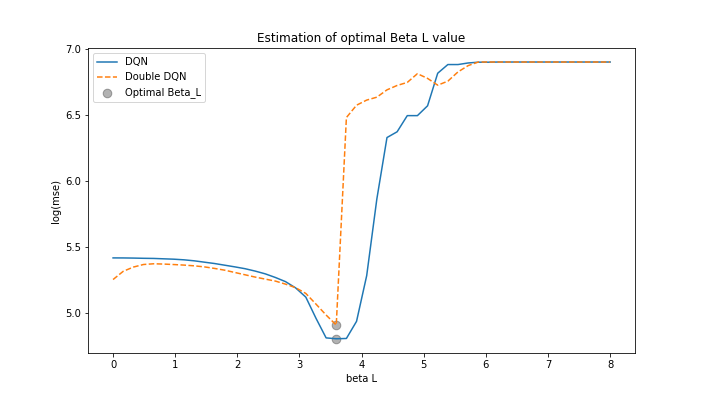
\includegraphics[width=1\linewidth]{figures/dqn_ddqn_model1_estimation_Beta_L.png}
  \caption{DQN and Double DQN estimation of $\beta_L$}
  \label{fig:dqn_ddqn_estimation_beta_L}
\end{subfigure}
    \caption{Estimation of $\beta_L$}
    \label{fig:beta_L_estimation}
\end{figure}

